So far, we have not done anything with \plumbing that you could not do in any other language. In this chapter, we will show you how you can use \plumbing to blink two LEDs at different speeds in {\em just four lines of code}. 

\GOALS
\begin{enumerate}
	\item Blink two LEDs together or separately.
	\item Learn about \PAR, the \occam construct for building \PARallel programs.
\end{enumerate}

\section{Build the circuit}
You may have modified things as part of your explorations in the last chapter. For Chapter~\ref{ch3}, you'll need two LEDs connected to your Arduino---one connected to pin \pineleven and one connected to pin \pintwelve. The cathode of each LED should be connected to ground through a resistor with a value between 470\ohm and 1k\ohm. Figure~\vref{circuit:ch3-two-led-circuit} shows how you should configure your Arduino.	

\begin{figure}[ht]
  \begin{center}
    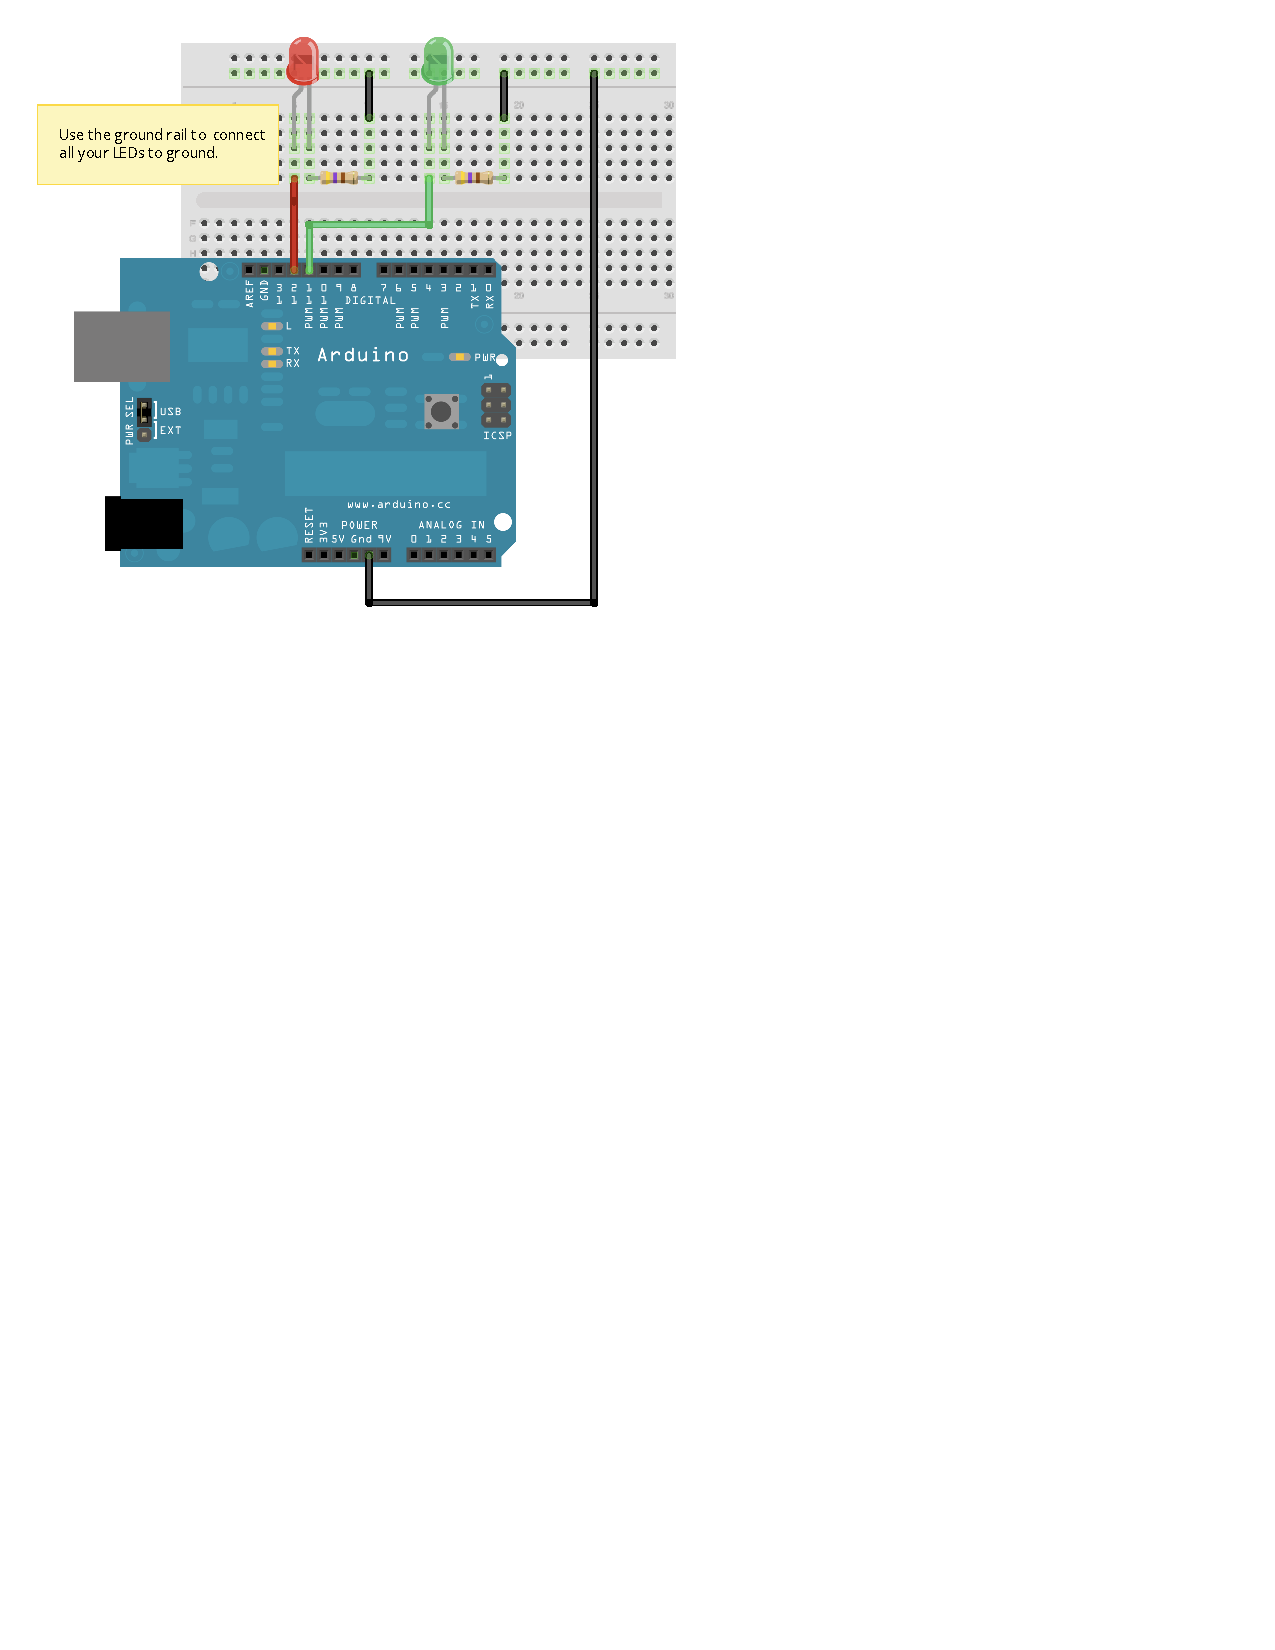
\includegraphics[width=0.8\linewidth]{images/ch3-two-led-circuit}
    \caption{A circuit connecting two LEDs to the Arduino.}
    \label{circuit:ch3-two-led-circuit}
  \end{center}
\end{figure}

In the previous chapter, we used \blink to turn one LED on and off at a rate of our choosing. Now, we don't want to blink just one LED, but instead want to blink two. Unlike many programming languages, \occam gives us a way of saying this directly. We can write a program that says ``please blink the LED on pin \pineleven at the same time as you blink the LED on pin \pintwelve.'' There is no other language available for the Arduino that lets you express this so simply.

\newpage

\CODE
\lstinputlisting[caption=We can {\procname blink} in \PARallel.,label=code:blink-par]{code/blink-par.occ}

\section{The \PAR pattern}

In the previous chapters, we've written a {\procname main} procedure that only did one thing. Many interesting programs need to do lots of things {\em at the same time}. If we want two things to happen at the same time, we use \PAR.

So far, we have seen that a \PROC may only contain one process, and that is indented by two spaces. To do two things simultaneously, then we need to use something like a \PAR. The \PAR itself is indented two spaces, and then everything underneath it is indented two more spaces. We can put {\em any number of additional processes} underneath a \PAR, and \occam will take care of running all of them in parallel. In the code in Listing~\vref{code:blink-par}, you can see that we are asking \plumbing to run two things in parallel, because there are two procedures underneath the \PAR. This pattern is illustrated in Figure~\vref{pattern:ch3-pattern-par}.

\begin{figure}[ht]
  \begin{center}
    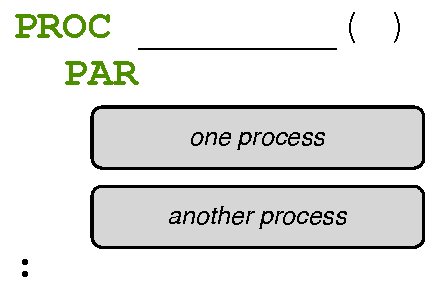
\includegraphics[width=0.6\linewidth]{images/ch3-pattern-par}
    \caption{Executing two processes in parallel.}
    \label{pattern:ch3-pattern-par}
  \end{center}
\end{figure}

	\newpage
	
As it happens, we are asking \plumbing to run two {\procname blink} processes. Our program asks it to blink the LED on pin \pintwelve at the same time as we blink the LED on pin \pineleven. Type in this new program and upload it to your Arduino; if all goes well, both LEDs should be blinking in synchrony.

\subsection{The truth about \PAR}


We have been saying that when you indent processes underneath a \PAR that they will happen ``at the same time.'' This is what it means when we say two things happen ``in parallel.'' However, your {\strong Arduino only has one processor}. It is typically the case that a device with only one processor can only do only do one thing at a time. Despite this, we are clearly executing a program that blinks two LEDs at the same time!

\newpage

\begin{figure}[ht]
%\begin{wrapfigure}{r}{0.45\linewidth}
  \begin{center}
    
\includegraphics[width=0.8\linewidth]{images/juggling}
		%\captionsetup{labelformat=empty,justification=centering,font=footnotesize}
    \caption{Parallel processes are juggled on the Arduino.}
    \label{image:juggling}
  \end{center}
%\end{wrapfigure}
\end{figure}

This may seem like an odd state of affairs: we wrote a program that blinks two LEDs in \PARallel, but the Arduino can only do one thing at a time. While \occam was originally designed so you could write programs that run on many processors, it can also be made to work just fine on a single processor. To make this possible, we wrote a piece of software called the Transterpreter\footnote{\url{http://www.transterpreter.org/}} that runs \occam programs and provides the illusion of parallelism by juggling all your parallel processes around, making sure each one gets a turn. 

The illusion of parallelism is called {\strong concurrency}. This should, we hope, provide a clue as to why our website's name is \url{concurrency.cc}! 



\EXPLORATIONS
It is likely that, at this point, you are chomping at the bit to do much more... you're now thinking about running motors, and sensors, and all kinds of things in parallel, doing things were never knew how to do before. For the moment, we're going to continue to explore \occam and the \plumbing library one step at a time.

Based on what we've done so far, you should be able to do some additional explorations on your own.

\begin{description}
	\item[Vary the parameters]\ \\
	Currently, both LEDs are blinking at the exact same rate. Try changing the rate at which they blink by varying the second parameter to the {\procname blink} process.
	\item[Add more LEDs]\ \\
	If you have more LEDs, you should be able to wire them up like your first LED using more pins on the Arduino. Then, add more {\procname blink} processes underneath the \PAR that will turn that pin on and off.
\end{description}

\subsection*{And a bit of science...}
If you have an oscilloscope, you can do some testing on your Arduino. How fast, for example, can you \blink an LED? Does {\code blink(13, 1)} really turn an LED on and off at a rate of 1ms? Or, is it slower than that? Record these numbers in your notebook, and see if you can work out the limit as to how quickly you can drive an LED on and off when using \plumbing.

\newpage

\BREAKAGE
There are a lot of neat ways to break the code in this chapter.

\begin{description}
		\item[Indentation of \PAR]\ \\
	What happens if you fail to indent \PAR, but indent all of the {\procname blink} procedures? We make this mistake in our code all the time.
		\item[Lowercase \PAR]\ \\
	What happens if you make {\strong par} all lowercase? What if you only capitalize the {\strong P}? 
	\item[Indentation of {\procname blink}]\ \\
	Try indenting each {\procname blink} process four spaces instead of two. What happens?
	\item[Multiple {\procname blink}s on one pin]\ \\
	Modify your program so that two of your {\procname blink} processes refer to the same pin number. (Note this breaks {\em after} you upload your program, not before!)
	\item[Replace one {\procname blink} with a {\procname heartbeat}]\ \\
	Modify your program so the \PAR looks like this:
	\begin{lstlisting}[firstnumber=2]
PAR
  heartbeat ()
  blink (11, 500)
	\end{lstlisting}
	What happens? Does this break anything? What if you \blink pin \pinthirteen instead of \pineleven?
	\item[Two \heartbeat processes]\ \\
	What happens if you run two \heartbeat processes in parallel?
\end{description}
	
